\section{Программная реализация}

\subsection{Описание области}
Задана область $$\Omega = \Omega_{01} \cup \Omega_{02} \cup \Omega_{11} \cup \Omega_{12} \cup \Omega_{10} \cup \Omega_{10} \cup \Omega_{20} $$.

Неизвестные функции: плотность $\rho$ и вектор скорости $\vec{u}$ являются функциями переменных Эйлера $(t, x) \in Q = [0, T] \times \Omega$.


\begin{figure}[h!] \centering
	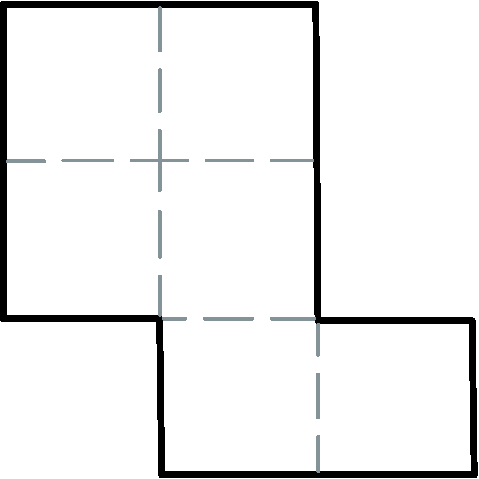
\includegraphics[scale=0.6]{area_1.pdf}
	\captionof{figure}{Заданная область}
\end{figure}


\subsection{Особенности реализации программы}
Система~\eqref{eq:system} является линейной относительно переменных $G^{n+1}$, $(V_s)^{n+1}$, $s = 1, \, \ldots, \, d$ с разреженной матрицей коэффициентов и, следовательно, может быть эффективно решена с помощью какого-либо итерационного алгоритма. В качестве же начального приближения можно взять значения на $n$-ом слое. \\

Для использования итерационных методов решения разреженных линейных систем матрицы стоит делать ближе к диагональной. Для этого необходимо упорядочить уравнения системы~\eqref{eq:system}. Зададим сперва на сетке $\omega_h$ порядок: нулевым узлом будем считать узел, имеющий наименьшие значения всех пространственных координат; далее последовательно выбираются узлы, у которых в первую очередь увеличивается первая координата, потом вторая и т.д., причем при изменении $s$-ой координаты, $s = 2, \, \ldots, \, d$, координаты $1, \, \ldots, \, s - 1$ принимают наименьшее возможное значение. Пронумеровав все узлы, обозначим $z = (\widehat{G}_0, \, (\widehat{V}_1)_0, \, (\widehat{V}_2)_0, \, \ldots, \, (\widehat{V}_d)_0, \, \widehat{G}_1, \, (\widehat{V}_1)_1, \, (\widehat{V}_2)_1, \, \ldots, \, (\widehat{V}_d)_1, \ldots)^T$. 
В результате получится система $Az=b$ с почти $3(d+1)$ диагональной матрицей $A$. \\

В случае $d = 2$ : $z = (\widehat{G}_0, \, (\widehat{V}_1)_0, \, (\widehat{V}_2)_0, \, 
                         \widehat{G}_1, \, (\widehat{V}_1)_1, \, (\widehat{V}_2)_1, \, \ldots)^T$.
Матрица почти 9-диагональная. \\

Для решения системы будем использовать стабилизированный метод бисопряжённых градиентов (англ. bi-conjugate gradient stabilized method, BiCGStab) с использованием ILUT (Incomplete LU with Threshold) предобусловливателя.
Реализация метода была взята из библиотеки Eigen (см. \cite{Eigen}), все параметры, кроме предобусловливателя, по умолчанию.


%\subsection{Особенности параллельной реализации программы}
%Параллельная реализация предобусловливателя, векторых и матричных операций не дали значительный прирост к времени работы программы. Связано это с тем, что большая часть времени уходит на заполнение матрицы и вектора правой части. Однако, стоит отметить, что параллелизм очень хорошо сказался на предобусловливателе, векторых и матричных операциях.
